\documentclass[t]{beamer}

\usetheme{TuringLight}
%\usetheme{TuringDark}

\usepackage{amsmath}
\usepackage{amssymb}
\usepackage{xspace}

\usepackage{multirow}
\usepackage{multicol}

\usepackage{subcaption}
%%Avoids error with subcaption...
\captionsetup{compatibility=false}
%%%
\usepackage{cite}

\newcommand{\ie}{\textit{i}.\textit{e}.,\xspace}
\newcommand{\eg}{\textit{e}.\textit{g}.,\xspace}

\newcommand{\ontoOne}{\ensuremath{\O_1}}
\newcommand{\ontoTwo}{\ensuremath{\O_2}}

\newcommand{\FMA}{\ensuremath{\O_\text{FMA}}}
\newcommand{\NCI}{\ensuremath{\O_\text{NCI}}}
\newcommand{\SNOMED}{\ensuremath{\O_\text{SNMD}}}

%For partitions
\newcommand{\ontoOneP}[1]{\ensuremath{\ontoOne}^{#1}}
\newcommand{\ontoTwoP}[1]{\ensuremath{\ontoTwo}^{#1}}



\newcommand{\ontoUnion}{\ensuremath{\O^{\M}}}
\renewcommand{\O}{\ensuremath{\mathcal{O}}\xspace}
\newcommand{\M}{\ensuremath{\mathcal{M}}}
\newcommand{\T}{\ensuremath{\mathcal{T}}}
\renewcommand{\P}{\ensuremath{\mathcal{P}}}
\newcommand{\D}{\ensuremath{\mathcal{D}}}
\newcommand{\mapping}[4]{\langle #1,\allowbreak #2,\allowbreak #3,\allowbreak #4
\rangle}
\newcommand{\mappingTwo}[2]{\langle #1,\allowbreak #2 \rangle}
\newcommand{\myset}[1]{ \{#1\} }
\newcommand{\MS}{\M^{S}\xspace}
\newcommand{\MRA}{\M^{RA}\xspace}
\newcommand{\MRAFN}{\MRA_{\text{fma-nci}}\xspace}
\newcommand{\MRAFS}{\MRA_{\text{fma-snmd}}\xspace}
\newcommand{\MRASN}{\MRA_{\text{snmd-nci}}\xspace}
\newcommand{\MLex}{\M^{\lex}\xspace}
\newcommand{\MT}{\ensuremath{\M\T}\xspace}
\newcommand{\MTLex}{\MT^{\lex}\xspace}
\newcommand{\PMT}{\ensuremath{\D_{\MT}}\xspace}
\newcommand{\MTM}{\MT^{\M}\xspace}
\newcommand{\MTMO}{\MT^{\M}_{\O_1\text{-}\O_2}\xspace}
\newcommand{\MTRAFN}{\MT^{RA}_{\text{fma-nci}}\xspace}

\newcommand{\cem}[1]{\mathsf{#1}}
\newcommand{\nsp}{\negthickspace}
\newcommand{\ntsp}{\negthinspace}
\newcommand{\nmsp}{\negmedspace}


\newtheorem{hypothesis}{Hypothesis}


\newcommand{\lexN}{\textsf{LexI}}
\newcommand{\lex}{\textsf{LexI}\xspace}
\newcommand{\starspace}{\textsf{StarSpace}\xspace}


% Definitions for algorithmic package
\newcommand{\logicalalgo}[1]{\ifmmode \text{ \textbf{#1} } \else \textbf{#1} \fi}
\newcommand{\notalgo}{\logicalalgo{not} }
\newcommand{\isnotalgo}{\logicalalgo{is not} }
\newcommand{\andalgo}{\logicalalgo{and}}
\newcommand{\oralgo}{\logicalalgo{or}}
\newcommand{\funcalgo}[1]{\ensuremath{\mathsf{#1}}}
\newcommand{\assignalgo}[2]{\State \ensuremath{#1 \leftarrow #2}}
\newcommand{\ForEach}[2]{\For{\textbf{ each } {#1} \textbf{ in } {#2} }}
\newcommand{\ForEachShort}[1]{\For{\textbf{ each } {#1} }}
\newcommand{\truealgo}{\ensuremath{\textsf{true}}}
\newcommand{\falsealgo}{\ensuremath{\textsf{false}}}
\newcommand{\continuealgo}{\textbf{continue}}
\newcommand{\breakalgo}{\textbf{break}}
\newcommand{\gotoalgo}[1]{\textbf{goto} line \ref{#1}}
\newcommand{\commentalgo}[1]{\Statex $\triangleright$ \textit{#1:}}


% Presentation data
\title{}
\subtitle{We Divide, You Conquer: From Large-scale Ontology Alignment to Manageable Subtasks}
\date{October 8, 2018}
\author{\textbf{Ernesto Jim\'enez-Ruiz}, Asan Agibetov, Matthias Samwald, Valerie Cross}

% Uncomment line below to set custom size for main slide text (default is 32pt)
%\setlength{\bodytext}{32pt}

% Start document
\begin{document}

% Title slide (details filled from presentation data fields above)
\begin{frame}
	\titlepage
\end{frame}

% Imprint slide (e.g. about the institute / opening quote)
%\begin{frame}
%	\imprintpage
%\end{frame}

% Section divider slide
\section{Introduction}



\begin{frame}{Motivation}

  		\begin{itemize}    
  			\item \textbf{Large-scale ontology matching} tasks is still \textbf{hard} for some systems
  			\item \textbf{Only 7} (out of 10) are able to \textbf{completed} all tasks in \textbf{Largebio} 2018 
  			\begin{itemize}
  			    \item \textit{6 hours timeout}
  			\end{itemize}
  			\item 14 (``all'') participants are able to complete Anatomy
  			\begin{itemize}
  			    \item \textit{5 systems focus on Complex, Multilingual or Instance tracks}
  			\end{itemize}
  			\item \textbf{Scalability and coverage guarantees} of state-of-the-art solutions
  		\end{itemize}
  	
\end{frame}


\begin{frame}{Motivation: prominent examples}

  		\begin{itemize}    
  			\item \textbf{YAM++ (2011):} best in \emph{conference}, but failed in
  			\emph{anatomy}.
            \item \textbf{CODI (2011.5):} best in \emph{anatomy}, but failed in
            \emph{largebio}.
            \item \textbf{MAMBA (2015):} top system in \emph{conference},
            but could not complete. \emph{anatomy}.
            \item<2-> \textbf{FCA-Map (2016):} failed to complete largest
            \emph{largebio} tasks.
            \item<2-> \textbf{POMap (2017):} top system in \emph{anatomy}, but
            could not finish largest \emph{largebio}.
            \item<2-> \textbf{ALOD2Vec (2018):} very good results in FMA-NCI
            small case, but could not complete the large case\textbf{}.
		\end{itemize}
  	
  	(*) With the available evaluation resources.
  	
\end{frame}



\begin{frame}{Preliminaries: matching task and evaluation measures}
	
  		\begin{itemize}    
  			\item An ontology \textbf{alignment} is a
set of mappings $\M$ between two ontologies $\O_1$ and $\O_2$.
			\item $m=\langle e_1, e_2 \rangle \in \M$ is a \textbf{mapping} with $e_1\in
			\O_1$ and $e_2\in \O_2$
  			\item<2-> An ontology \textbf{matching task} $\MT$:
  				\begin{itemize} 
  				  \item a pair of ontologies $\O_1$ (source) and $\O_2$ (target) 
  				  \item (optional) \textbf{reference alignment} $\MRA$
  				 \end{itemize}
  			\item<2-> The \textbf{size} or \textbf{search space} of a matching task:
  			$\lvert Sig(\O_1) \rvert \times \lvert Sig(\O_2) \rvert$
  			
  			\item<3-> \textbf{Matching system}: given $\O_1$ and $\O_2$ produces $\MS$
  			\item<3-> The standard \textbf{evaluation measures}:
  			\begin{equation*}
    P = \frac{\lvert\MS \cap \MRA\rvert}{\lvert\MS\rvert},~
    R = \frac{\lvert\MS \cap \MRA\rvert}{\lvert\MRA\rvert},~
    F = 2 \cdot \frac{P \cdot R}{P + R} 
\end{equation*}
		\end{itemize}
  	
\end{frame}



\begin{frame}{Preliminaries: Division and Matching subtasks}
	
  		\begin{itemize}    
  		 
  		  \item \emph{Division} of a matching task $\MT$ (composed by
$\O_1$ and $\O_2$) 
		\begin{itemize}
%as the process of finding matching subtasks 
			\item process of finding matching subtasks: \\
			$\PMT^{n}=\{\MT_1,\ldots,\MT_n\}$
			\item where $\MT_{i}=\langle \ontoOne^{i}, \ontoTwo^{i} \rangle$ and  $\ontoOne^{i} \subset \ontoOne$ and $\ontoTwo^{i} \subset
\ontoTwo$. 
		\end{itemize}
  	
  	
		\end{itemize}
  	
\end{frame}



\begin{frame}{Preliminaries: desired guarantess}
	
	\begin{block}{Size ratio < 1.0}
	
	\begin{equation*}
    	\funcalgo{SizeRatio}(\MT_i, \MT) = \frac{\lvert Sig(\ontoOne^{i}) \rvert
    	\times \lvert Sig(\ontoTwo^{i}) \rvert} {\lvert Sig(\O_1) \rvert \times
    	\lvert Sig(\O_2)\rvert}
	\end{equation*}

	\begin{equation*}
    	\funcalgo{SizeRatio}(\PMT^{n}, \MT) =
    	\sum_{i=1}^{n}\funcalgo{SizeRatio}(\MT_i, \MT)
	\end{equation*}
	
	
	\end{block}
	
  	
  	\begin{block}<2->{Coverage ratio $\approx$ 1.0}
  	
  	$m\in\M$ is covered by a division $\PMT^{n}$  if $m$ ca be dicovered in
  	on (or more) $\MT_i$
  	
	  	\begin{equation*}
	    \funcalgo{CoverageRatio}(\PMT^{n}, \M) =
	    \frac{\lvert\funcalgo{Coverage}(\PMT, \M)\rvert} {\lvert \M \rvert}
		\end{equation*}
  	\end{block}
  	
  		%\begin{itemize}    
  		%	\item Basic definitions
  		%	\item Guarantees
  		%	\item Hypothesis?
		%\end{itemize}
  	
\end{frame}


\section{Methods}





\begin{frame}{Methods: lexical index \lex}
	
	\begin{itemize}
	  \item \lex indexes de vocabulary of the ontologies
	  \item Entries in \lex are a source of mappings (\ie $\MLex$)
	  \item<2-> $\MLex$ is a manageable (approximation) of the Cartesian product
	  \item<2-> $\MLex$ represents an upper-bound of (most) system-computed
	  mappings
	\end{itemize}
	
	
	
	\centering
{
%\begin{footnotesize}

\begin{tabular}{ll}
\begin{footnotesize}
%\begin{scriptsize}
\begin{tabular}[t]{|l||l|l|}
\hline 

\multirow{2}{*}{\textbf{Index key}} & \multicolumn{2}{c|}{\textbf{Index value}}
\\\cline{2-3} 
& \textbf{Entities $\ontoOne$} & \textbf{Entities $\ontoTwo$} \\\hline

$\{$ acinus $\}$ & 7661,8171 & 118081 \\\hline

%$\{$ small, intestin, lieberkuhn $\}$ & 31465 & 82989 \\\hline
$\{$ mesothelial, pleural $\}$ & 19987 & 117237 \\\hline
 \multicolumn{3}{c}{\tiny{~}\vspace{-0.21cm}} \\\hline

$\{$ hamate, lunate $\}$ & 55518 & - \\\hline

$\{$ feed, breast $\}$ & - & 113578,111023 \\\hline


%[small, intestin, lieberkuhn]%
	%31465 
	% http://bioontology.org/projects/ontologies/fma/fmaOwlDlComponent_2_0#Crypt_of_Lieberkuhn_of_small_intestine
		%82989 
	% http://ncicb.nci.nih.gov/xml/owl/EVS/Thesaurus.owl#Small_Intestinal_Crypt_of_Lieberkuhn


%Lunate_facet_of_hamate


%}
\end{tabular}
%\end{scriptsize}
\end{footnotesize}
&
\begin{scriptsize}
\begin{tabular}[t]{|l||l|}
\hline 
\textbf{ID} & \textbf{URI} \\\hline
7661 & \ontoOne:Serous\_acinus \\
8171 & \ontoOne:Hepatic\_acinus \\
19987 & \ontoOne:Mesothelial\_cell\_of\_pleura\\
55518 & \ontoOne:Lunate\_facet\_of\_hamate\\\hline
118081 & \ontoTwo:Liver\_acinus \\
117237 & \ontoTwo:Pleural\_Mesothelial\_Cell\\
%31465 & Crypt\_of\_Lieberkuhn\_of\_small\_intestine\\
%82989 & Small\_Intestinal\_Crypt\_of\_Lieberkuhn\\
113578 & \ontoTwo:Breast\_Feeding\\
111023 & \ontoTwo:Inability\_To\_Breast\_Feed\\\hline

\end{tabular}
\end{scriptsize}
\end{tabular}



%\end{footnotesize}
}

	
	
\end{frame}




\begin{frame}{Methods: context as matching task}
	
	\begin{block}{Locality modules}
	
	Logic-based modules capture the \textbf{semantically related entites (context)}
	for a given signature and ontology.
	\end{block}
	
	\begin{block}<2->{Context of an alignment}
	
	The context of $\M$ (between $\O_1$ and $\O_2$) is composed by two modules
	$\O_1'$ and $\O_2'$
	
	
	\end{block}
	
	
	
	\begin{block}<3->{Context as matching task}
	
	
	A task $\MT=\langle \O_1, \O_2 \rangle$ to find $\M$ can be reduced to
	$\MT'=\langle \O_1', \O_2' \rangle$
	
	\end{block}
	
	
	
  	
\end{frame}



\begin{frame}{Methods: from \lex to matching (sub)task(s)}

\begin{block}{Context of $\MLex$ as mathcing task}

\begin{itemize}
  \item $\MLex$ leads to a mathcing (sub)task $\MTLex=\langle \O_1', \O_2' \rangle$
with $\O_1' \subseteq \O_1$ and $\O_2' \subseteq \O_2$
  \item $\O_1'$ and $\O_2'$ may still be large for some systems 
\end{itemize}

\end{block}


%\vfill
\begin{block}<2->{Solution: cluster \lex}
\includegraphics[width=1.0\textwidth]{figures/workflow_clustering.png}
\end{block}

\end{frame}



\begin{frame}{Methods: clustering}
	
	\begin{block}{Naive strategy}
		Random split of \lex into a number of cluster of the same size.
	\end{block}
	
	
	\begin{block}<2->{Neural embedding strategy}
	\begin{itemize}
	  \item It relies on StarSpace tookit and neural embedding model
	  \item We learn embeddings for the words in the keys of \lex
	  \item \textbf{\lex key embeddings}: Mean vector of the single word 
	  embeddings 
	  %%Why not mean of the entities in the values!!! 
	  %%Or a combination?? 
	  %%Check if subsumption is somehoe kept
	  \item Standard clustering with the K-means algorithm
	\end{itemize}
	
	\end{block}
	
	
  	
\end{frame}





% \begin{frame}{Methods}
% 	
% 		\begin{itemize}
%   		  	\item Locality    
%   			\item Lexical index
%   			\item Pipeline
%   			\item Division
%   			\item Division as in LogMap
%   			\item Multiple division
% 		\end{itemize}
%   	
% \end{frame}
% 
% 



\section{Evaluation}



\begin{frame}{Evaluation setting}

\begin{itemize}
  \item Datasets and systems of the OAEI campaigns
  \item 
Ubuntu Laptop with an Intel Core i7-4600U CPU@2.10GHz (4 cores). Up to 15 Gb of
RAM was allocated.
\end{itemize}



	\centering
{
\begin{footnotesize}
\begin{tabular}{|c|c|c||c|c|c|}

\hline
\textbf{OAEI track} & \textbf{Source of $\MRA$} & \textbf{Task}  &
\textbf{Ontology} & \textbf{Version} & \textbf{Size (classes)} \\\hline\hline

\multirow{2}{*}{Anatomy} &  \multirow{2}{*}{Manually
created} & \multirow{2}{*}{AMA-NCIA} & AMA & v.2007 & 2,744 \\
& & & NCIA & v.2007 & 3,304 \\\hline\hline

\multirow{3}{*}{Largebio} & \multirow{3}{*}{UMLS-Metathesaurus} & FMA-NCI & FMA
& v.2.0 & 78,989 \\
& & ~FMA-SNOMED~ & NCI & v.08.05d &  66,724 \\
& & SNOMED-NCI & ~SNOMED~ &  v.2009 &  306,591\\\hline\hline


\multirow{4}{*}{Phenotype} & 
%\multirow{4}{*}{Consensus alignment (vote=2)} 
\multirow{4}{*}{\vtop{\hbox{\strut Consensus alignment}\hbox{\strut (vote=2)
}}}

& \multirow{2}{*}{HPO-MP} & HPO &
~v.2016-BP~ & 11,786 \\
& & & MP & v.2016-BP & 11,721 \\
& &  \multirow{2}{*}{DOID-ORDO} & DOID & v.2016-BP & 9,248 \\
& & & ORDO & v.2016-BP & 12,936 \\\hline

\end{tabular}
\end{footnotesize}
}
	
  	
\end{frame}





\begin{frame}{Evaluation: adequacy in terms of \emph{size ratio} }
	
	
	\begin{figure}[t]
    \centering
    \begin{subfigure}[b]{0.495\textwidth}
        \centering
        \includegraphics[width=\textwidth]{figures/ratios.eps}\\[-1ex]
        \caption{Naive strategy}
        \label{fig:ratioN}
    \end{subfigure}
    %\hfill
    \begin{subfigure}[b]{0.495\textwidth}
        \centering
        \includegraphics[width=\textwidth]{figures/ratios_advanced.eps}\\[-1ex]
        \caption{Neural embedding strategy}
        \label{fig:ratioA}
    \end{subfigure}
    
\end{figure}
  		
  	
\end{frame}



\begin{frame}{Evaluation: cloud of sizes in AMA-NCIA }
	
\begin{figure}[t]
    \centering
    \begin{subfigure}[b]{0.495\textwidth}
        \centering
        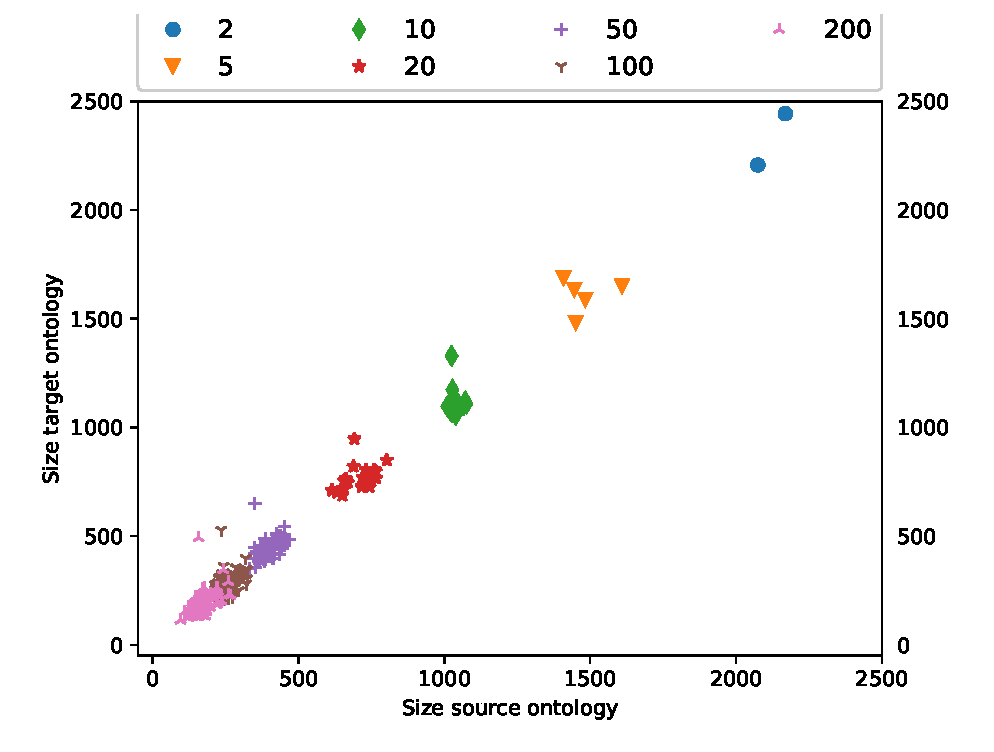
\includegraphics[width=\textwidth]{figures/cloud_mouse_naive.eps}\\[-1ex]
        \caption{Naive strategy}
        \label{fig:mouse-naive}
    \end{subfigure}
    %\hfill
    \begin{subfigure}[b]{0.495\textwidth}
        \centering
        \includegraphics[width=\textwidth]{figures/cloud_mouse_advanced.eps}\\[-1ex]
        \caption{Neural embedding strategy}
        \label{fig:mouse-advanced}
    \end{subfigure}
\end{figure}

\end{frame}

\begin{frame}{Evaluation: cloud of sizes in FMA-NCI }
	\begin{figure}[t]
    \centering
    \begin{subfigure}[b]{0.495\textwidth}
        \centering
        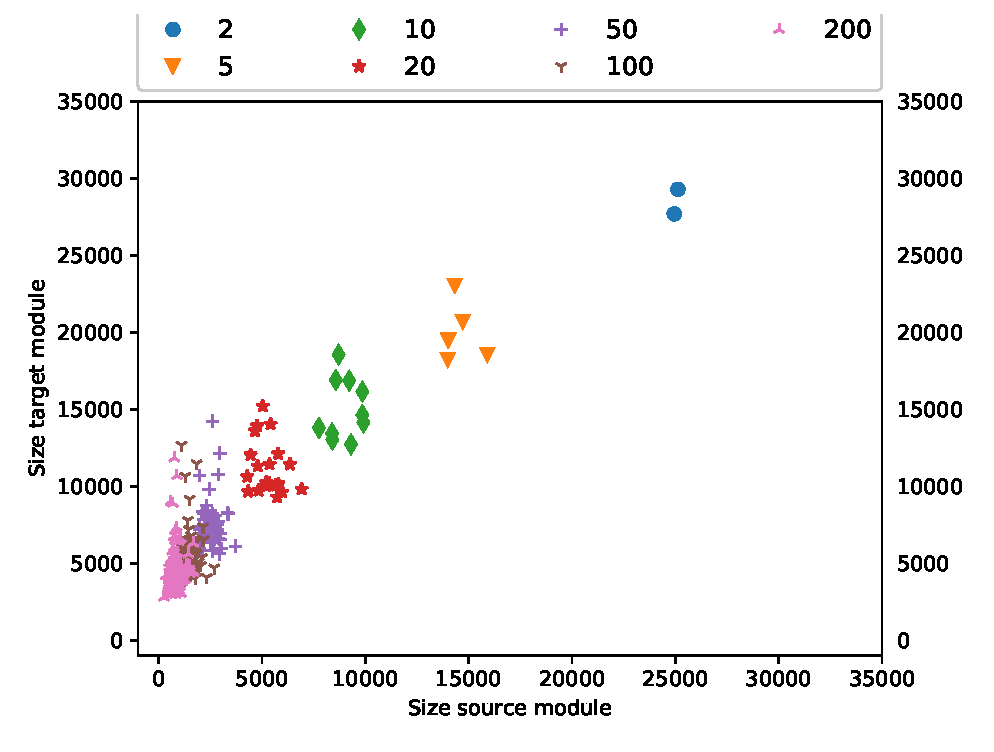
\includegraphics[width=\textwidth]{figures/cloud_fma2nci_naive.eps}\\[-1ex]
        \caption{Naive strategy}
        \label{fig:f2n-naive}
    \end{subfigure}
    %\hfill
    \begin{subfigure}[b]{0.495\textwidth}
        \centering
        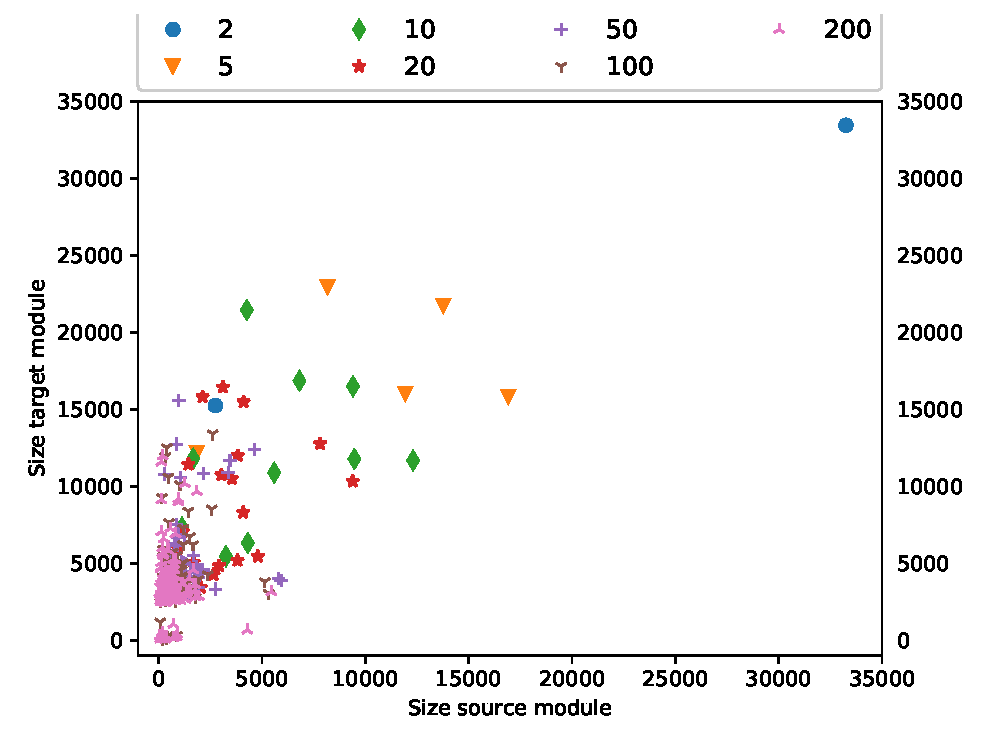
\includegraphics[width=\textwidth]{figures/cloud_fma2nci_advanced.eps}\\[-1ex]
        \caption{Neural embedding strategy}
        \label{fig:f2n-advanced}
    \end{subfigure}

\end{figure}	
  	
\end{frame}



\begin{frame}{Evaluation: adequacy in terms of \emph{coverage ratio} }

\vspace{-0.1cm}
{\footnotesize (*) Coverage with respect to reference alignment}

	\begin{figure}[t]
    \centering
    \begin{subfigure}[b]{0.495\textwidth}
        \centering
        \includegraphics[width=\textwidth]{figures/coverages.eps}\\[-1ex]
        \caption{Naive strategy}
        \label{fig:coverageN}
    \end{subfigure}
    %\hfill
    \begin{subfigure}[b]{0.495\textwidth}
        \centering
        \includegraphics[width=\textwidth]{figures/coverages_advanced.eps}\\[-1ex]
        \caption{Neural embedding strategy}
        \label{fig:coverageA}
    \end{subfigure}
 \end{figure}

  	
\end{frame}



\begin{frame}{Evaluation: OAEI systems evaluation}
	
	Systems failing to complete tasks in the OAEI
2015-2017 campaigns.

	\vspace{0.4cm}
	
	{
\centering

\begin{scriptsize}
\begin{tabular}{|c|c|c|c||c|c|c|c||c|c|c|c|}
\hline

\multirow{2}{*}{\textbf{Tool}} & \multirow{2}{*}{\textbf{Task}} & 
\multirow{2}{*}{\textbf{Year}}
& 
%\multirow{2}{*}{\textbf{Partition}
\textbf{Matching} 
& \multicolumn{4}{c||}{\textbf{Naive
strategy}} & \multicolumn{4}{c|}{\textbf{Neural embedding
strategy}}\\\cline{5-12}

& & & \textbf{subtasks} &
~\textbf{P}~ &
~\textbf{R}~ &  ~\textbf{F}~ &  ~\textbf{t (h)~} &
~\textbf{P}~ &
~\textbf{R}~ &  ~\textbf{F}~ &  ~\textbf{t (h)~}
\\\hline\hline

\multirow{2}{*}{GMap (*)} & \multirow{2}{*}{Anatomy} & \multirow{2}{*}{2015} 
& 5 & 0.87 & 0.81 & \textbf{0.84} & 1.3 & 0.88 & 0.82 & \textbf{0.85} & 0.7\\
& & & 10 & 0.85 & 0.81 & \textbf{0.83} &	1.7 & 0.86 & 0.82 & \textbf{0.84} & 0.8
\\\hline\hline

\multirow{2}{*}{MAMBA} & \multirow{2}{*}{Anatomy} & \multirow{2}{*}{2015} & 
20 & ~0.88~ & ~0.63~ & ~\textbf{0.73}~ & 2.3 & ~0.89~ & ~0.62~ & ~\textbf{0.73}~ & 1.0  \\
& & & 50 & 0.88 & 0.62 & \textbf{0.73} & 2.4 & 0.89 & 0.62 &\textbf{ 0.73} & 1.0
\\\hline\hline


\multirow{2}{*}{FCA-Map} & \multirow{2}{*}{FMA-NCI} & \multirow{2}{*}{2016} 
& 20 & 0.56 & 0.90 & \textbf{0.72} & 4.4 &  0.62 & 0.90 & \textbf{0.73} & 3.1 \\
& & & 50 & 0.58 & 0.90 & \textbf{0.70} &	4.1 & 0.60 & 0.90 & \textbf{0.72} & 3.0 \\\hline\hline


\multirow{2}{*}{KEPLER} & \multirow{2}{*}{FMA-NCI} & \multirow{2}{*}{2017} 
& 20 & 0.45 & 0.82 & \textbf{0.58} & 8.9 & 0.48 & 0.80 &	\textbf{0.60} & 4.3\\
& & & 50 & 0.42 & 0.83 & \textbf{0.56} & 6.9 & 0.46 & 0.80 & \textbf{0.59} & 3.8
\\\hline\hline

\multirow{2}{*}{POMap} & \multirow{2}{*}{FMA-NCI} & \multirow{2}{*}{2017} 
& 20 & 0.54 & 0.83 & \textbf{0.66} &	11.9 & 0.56 & 0.79 & \textbf{0.66} & 5.7\\ 
& & & 50 & 0.55 & 0.83 & \textbf{0.66} & 8.8 & 0.57 & 0.79 & \textbf{0.66} & 4.1 \\\hline

%SANOM? & & & & & & & & & & &\\\hline
 
\end{tabular}
\end{scriptsize}
}
	
	{\scriptsize (*)Evaluated with 8Gb}
  		
\end{frame}



% \begin{frame}{Evaluation: adequacy in terms of size ratio }
% 	
%   		\begin{itemize}    
%   			\item Datasets OAEI
%   			\item Adequacy of clustering
%   			\item OAEI evaluation
%   			\item Impact on top systems?
%   			\item Availability: system, datasets...
% 		\end{itemize}
%   	
% \end{frame}






\section{Conclusions and Future Work}



\begin{frame}{Conclusions}



\begin{itemize}
  
  \item Evaluation of \textbf{coverage} and \textbf{size} before computing
  F-scores  %Related
  
  \item \textbf{Suitability} of using \textbf{\lex} and clustering strategies
  	\begin{itemize}
  	  	\item[+] simple and efficient approach 
  		\item[+] high coverage (i.e., minimal information loss)
  		\item[+] reduction of search space (apart from SNOMED-NCI)
  		\item[+] 5 OAEI systems managed to complete results
	\end{itemize}
	
	%\item System, source codes and datasets available online
	
\end{itemize}


\end{frame}





\begin{frame}{Future work}
  	
  	  \begin{itemize}    
  			\item \textbf{Estimation} of the number of \textbf{clusters} according to
  			systems and resources.
  			\item \textbf{Extension} of the conducted \textbf{evaluation}.
			\begin{itemize}
			  \item Impact on systems
			  \item Other notions of context
			  \item Other clustering approaches 
  			\end{itemize} 
		\end{itemize}
  	
\end{frame}








% End slide 
\begin{frame}{Questions?}
	
	
	Main contact:
	Ernesto Jimenez Ruiz (\url{ejimenez-ruiz@turing.ac.uk})
	\url{https://www.turing.ac.uk/people/researchers/ernesto-jimenez-ruiz}
	\\~\\
	Sources, datasets, paper: 
	~~~\url{https://github.com/ernestojimenezruiz/logmap-matcher}
	
	\vspace{1.1cm}
	
	\includegraphics[height=1.4\gridblock]{\logofilename}~~
	\includegraphics[height=1.4\gridblock]{images/sirius-logo.png}
	\\~~\\
	\includegraphics[height=1.0\gridblock]{images/muo.jpg}~~
	\includegraphics[height=1.2\gridblock]{images/muv.jpg}
		    
	\finalpage 
\end{frame}

\end{document}